\documentclass{article}

\usepackage[T1]{fontenc}
\usepackage[utf8]{inputenc}
\usepackage{lmodern}
\usepackage[obeyspaces,spaces]{url}
\usepackage{array}
\usepackage{tikz}
\usetikzlibrary{arrows.meta}
\usepackage{hyperref}

% Inline code is typeset like a URL: identifiers need no escaping, spaces
% are kept, and lines may break at spaces, underscores, dots and slashes.
\DeclareUrlCommand\code{\urlstyle{tt}}

% Ragged-right paragraph column for tables.
\newcolumntype{L}[1]{>{\raggedright\arraybackslash}p{#1}}

% Lets TeX stretch a line a little more before letting long identifiers
% stick out into the margin.
\setlength{\emergencystretch}{3em}

\title{clusterd\\[1ex]
  \large Design, wire protocol, operations and limitations\\
  Phase~1: heartbeat and status}
\author{}
\date{7 November 2026}

\begin{document}

\maketitle

\begin{abstract}
clusterd pools a small number of Linux machines so that independent
simulation runs can be submitted from one place and placed on whichever
machine has free capacity, and so that their disks can later be combined
into redundant shared storage. This document describes the system as
implemented at the end of Phase~1: one agent binary that runs on every
machine, a mutually authenticated TLS control channel rooted in a
cluster-private certificate authority, periodic heartbeats carrying CPU,
memory and disk figures, and a \code{clusterd status} command that shows
which machines are up. It explains the reasoning behind each design
choice, gives the complete wire-protocol reference and the procedure for
deploying on real machines, and then sets out in detail what the current
design does not do, what it does poorly, and the defects found and fixed
while writing it.
\end{abstract}

\tableofcontents

% ======================================================================
\section{Introduction}
% ======================================================================

\subsection{Purpose}

clusterd bundles several modest Linux machines into one pooled system
administered from a single place. Two capabilities are wanted:

\begin{itemize}
  \item \emph{Job pooling}: submit simulation jobs from one place and have
    each one placed on whichever machine has free capacity.
  \item \emph{Storage pooling}: combine the disks of all machines into one
    storage space with parity-based redundancy (``RAID~5'' semantics:
    losing one disk or one machine loses no data).
\end{itemize}

Three constraints shape everything else. The simulation code must run
unmodified. The system is administered entirely over SSH. And it must
feel like one system, not like a fleet of machines managed one by one.

The project starts as a prototype but is meant to grow into a production
system in an environment where failure has a real cost. That does not
change the incremental approach --- a small, well-tested foundation is the
stable way to start --- but it raises the bar within each increment:
thorough tests from the first phase, careful handling of every byte that
arrives from the network, and no privilege or assumption that would be
hard to walk back later.

\subsection{Non-goals}

clusterd does not try to make several machines look like one computer to
a single unmodified process (transparent distributed shared memory, or
CPU pooling across machines). That was the original request. The actual
workload --- CPU-bound, needing more memory than one machine has, running
in a managed runtime --- rules it out for any lightweight system. The
technologies that really do this are either proprietary hypervisor-level
products that need specialised RDMA hardware (ScaleMP, TidalScale) or
research systems that are abandoned and were never fast (Kerrighed,
openMosix).

The goal was therefore reframed to what is tractable without touching the
simulation code: job-level parallelism (many independent runs spread
across machines) plus pooled, redundant storage. One consequence must be
understood by every user: \emph{a single simulation run is still limited
to the CPU and memory of the one machine it runs on.} clusterd shortens
the time to finish a batch of runs; it does not make an individual run
faster or let it use more memory.

\subsection{Scope of this document}

This document covers Phase~1 as implemented, the phases planned after it,
and --- in detail --- the current limitations
(Section~\ref{sec:limitations}). Section~\ref{sec:defects} records the
defects found while writing it and how they were fixed. Whenever the
text says ``planned'' or names
a later phase, the corresponding code does not exist yet.

This is an engineering description, not a security audit or a
certification. Before clusterd carries real weight in a critical
environment, it needs a dedicated security and reliability review.

% ======================================================================
\section{Design principles}
% ======================================================================

\subsection{Delegate to proven tools}

Wherever a proven tool already solves a problem correctly, clusterd
delegates to it. From-scratch Rust is written only for the coordination
logic that is specific to this project. Table~\ref{tab:delegation} lists
the delegations, including those planned for later phases.

\begin{table}[htbp]
  \centering
  \begin{tabular}{L{0.26\textwidth}L{0.17\textwidth}L{0.35\textwidth}c}
    \hline
    Problem & Delegated to & clusterd's own job & Phase \\
    \hline
    Encryption and mutual authentication of the control channel
      & rustls (ring backend)
      & Create a small cluster CA and one certificate per machine
      & 1 \\
    CPU, memory and disk figures
      & \code{sysinfo} crate
      & Sample on every heartbeat and report to the head
      & 1 \\
    Process supervision and start at boot
      & systemd
      & Generate unit files, enable and start them, poll their status
      & 3 \\
    Remote authentication and first contact with a new machine
      & system \code{ssh} and \code{scp}
      & Invoke them; never reimplement SSH
      & 3 \\
    Redundant distributed storage
      & SeaweedFS (\code{weed})
      & Generate its configuration, run it under systemd, choose
        redundancy settings
      & 4 \\
    \hline
  \end{tabular}
  \caption{Problems delegated to existing tools.}
  \label{tab:delegation}
\end{table}

\subsection{Small, complete increments}

Distributed systems do not work as one giant first commit. Each phase
lands as a complete, working, tested increment rather than as part of a
large, partially working system (Table~\ref{tab:phases}).

\begin{table}[htbp]
  \centering
  \begin{tabular}{L{0.32\textwidth}L{0.13\textwidth}L{0.43\textwidth}}
    \hline
    Phase & Status & Delivers \\
    \hline
    0 --- workspace skeleton & Done
      & Cargo workspace with the three crates \\
    1 --- heartbeat and status & Done
      & Agent runtime, mutual TLS, live node table, \code{clusterd init},
        \code{clusterd cert issue}, \code{clusterd status} \\
    2 --- job submission and scheduling & Not started
      & \code{clusterd run}, placement, log streaming, job persistence \\
    3 --- automated node join & Not started
      & One-command onboarding over SSH, systemd unit installation \\
    4 --- storage orchestration & Not started
      & Pooled redundant storage on SeaweedFS, FUSE mount \\
    \hline
  \end{tabular}
  \caption{Phases and their status.}
  \label{tab:phases}
\end{table}

\subsection{One binary; the role is configuration}

Every machine, the head included, runs the same command,
\code{clusterd agent run}. Whether a machine is the head or a worker is a
single field in its \code{config.toml}, not a different program. The head
is a superset of a worker: it contributes its own CPU, memory and disk to
the pool exactly like a worker, and in addition it accepts connections
from workers, keeps the node table, and serves the local control socket
used by the command-line interface. From Phase~2 it will also run the
scheduler.

This leaves one artifact to build, copy and upgrade, and head and workers
cannot drift apart in behaviour.

\subsection{Pure logic kept apart from input and output}

The node table --- the code that decides whether a machine is up --- does
no networking and no sleeping. Its test-facing methods take the current
time as a parameter (\code{record_heartbeat_at}, \code{snapshot_at}), so
the behaviour at the timeout boundary is tested deterministically against
a fabricated clock. The networking code in \path{agent.rs} is kept as
thin wiring around such pure parts.

\subsection{No dependency or state before it is needed}

Phase~1 has no database. Nothing needs to survive a restart except the
configuration and the certificates, and the node table correctly rebuilds
itself from incoming heartbeats. SQLite (through \code{rusqlite}) arrives
with Phase~2, which has job history and a queue worth persisting; adding
it earlier would mean an unused dependency. The same reasoning rejected
gRPC and QUIC (Section~\ref{sec:transport}).

The release profile enables link-time optimisation, a single code
generation unit and symbol stripping, producing one compact executable.

% ======================================================================
\section{Architecture}
% ======================================================================

\subsection{Crates}

The Cargo workspace has three crates. Dependencies point in one direction
only: \code{clusterd} depends on \code{clusterd-core}, which depends on
\code{clusterd-proto}.

\begin{description}
  \item[\code{clusterd-proto}] The cross-machine contract: the
    \code{Message} enum and its framing. It has no opinion about the async
    runtime beyond the codec trait of \code{tokio-util}. Keeping it
    separate keeps the contract small, reviewable and testable in
    isolation, including by fuzzing.
  \item[\code{clusterd-core}] Everything else, as a library: agent
    runtime, TLS and identity, node table, resource sampling, local
    control protocol and configuration.
  \item[\code{clusterd}] The command-line program, built with
    \code{clap}; thin wiring over \code{clusterd-core}.
\end{description}

\subsection{Modules of clusterd-core}

\begin{description}
  \item[\code{config}] The TOML configuration (\code{node_id},
    \code{node_name}, \code{role}, \code{listen_addr} or
    \code{head_addr}, heartbeat interval and timeout) and the file layout
    of the data directory. Validation only checks that a head has a
    listen address and a worker has a head address.
  \item[\code{identity}] Generation of the cluster CA and of per-machine
    certificates with \code{rcgen}.
  \item[\code{tls}] Builds the rustls server and client configurations
    for mutual TLS from PEM files, and installs the ring crypto provider
    once per process.
  \item[\code{nodes}] The node table: records heartbeats and decides up or
    down. Pure and synchronous.
  \item[\code{resources}] CPU, memory and disk sampling through
    \code{sysinfo}.
  \item[\code{agent}] The runtime: the head's listener and per-connection
    handling, the head's own heartbeat, and the worker's connect, heartbeat
    and reconnect loop.
  \item[\code{ipc}] The local protocol between the command-line program
    and the agent on the same machine, over a Unix-domain socket.
  \item[\code{error}] One flat error type for the whole crate.
\end{description}

\subsection{Runtime structure}

Figure~\ref{fig:topology} shows the processes and tasks at run time.

\begin{figure}[htbp]
  \centering
  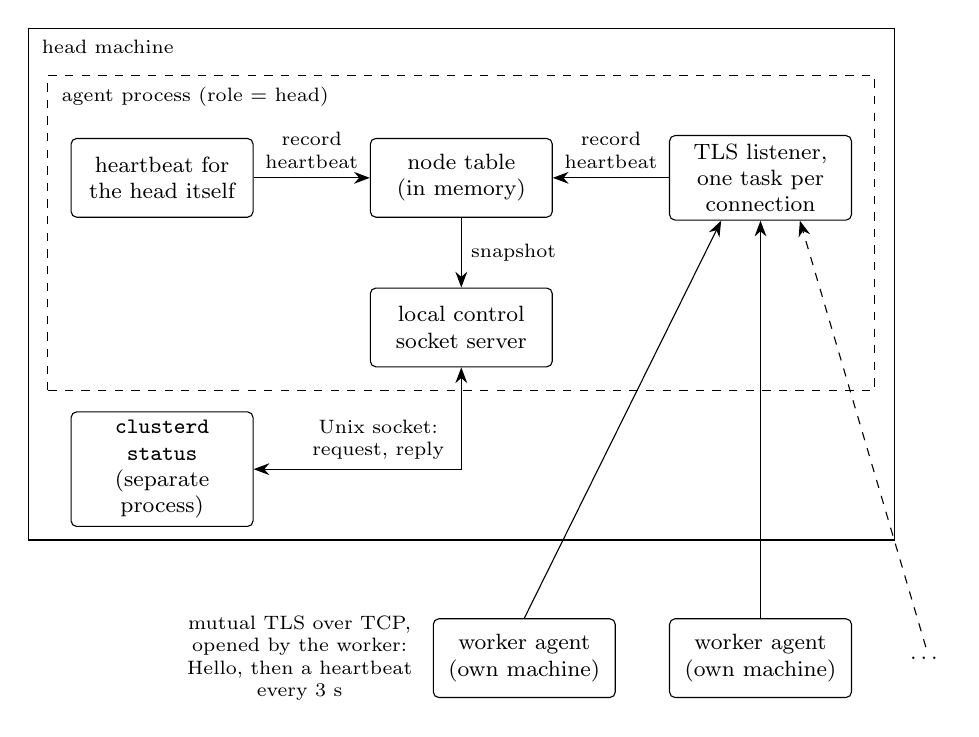
\begin{tikzpicture}[
      font=\footnotesize,
      >={Stealth[length=2mm]},
      comp/.style={draw, rounded corners=2pt, align=center,
                   text width=2.1cm, minimum height=1cm, inner sep=3pt},
      lbl/.style={font=\scriptsize, align=center}]
    % Head agent process
    \node[comp] (self)  at (0,0)     {heartbeat for\\the head itself};
    \node[comp] (table) at (3.8,0)   {node table\\(in memory)};
    \node[comp] (conn)  at (7.6,0)   {TLS listener,\\one task per\\connection};
    \node[comp] (uds)   at (3.8,-1.9){local control\\socket server};
    \draw[dashed] (-1.45,-2.7) rectangle (9.05,1.3);
    \node[lbl, anchor=north west] at (-1.4,1.28) {agent process (role = head)};
    % CLI on the head machine
    \node[comp] (cli)   at (0,-3.7)  {\texttt{clusterd status}\\(separate process)};
    \draw (-1.7,-4.6) rectangle (9.3,1.9);
    \node[lbl, anchor=north west] at (-1.65,1.88) {head machine};
    % Workers
    \node[comp] (w1) at (4.6,-6.1) {worker agent\\(own machine)};
    \node[comp] (w2) at (7.6,-6.1) {worker agent\\(own machine)};
    \node (wn) at (9.7,-6.1) {\dots};
    % Arrows
    \draw[->] (self) -- node[lbl, above] {record\\heartbeat} (table);
    \draw[->] (conn) -- node[lbl, above] {record\\heartbeat} (table);
    \draw[->] (table) -- node[lbl, right] {snapshot} (uds);
    \draw[<->] (cli.east) -| node[lbl, above, pos=0.3]
      {Unix socket:\\request, reply} (uds.south);
    \draw[->] (w1.north) -- ([xshift=-5mm]conn.south);
    \draw[->] (w2.north) -- (conn.south);
    \draw[->, dashed] (wn.north) -- ([xshift=5mm]conn.south);
    \node[lbl, anchor=east] at (3.3,-6.1)
      {mutual TLS over TCP,\\opened by the worker:\\Hello, then a heartbeat\\every 3 s};
  \end{tikzpicture}
  \caption{Run-time structure. Solid arrows into the node table are
    writes; the control socket only reads a snapshot. Workers always open
    the connection; the head never dials out.}
  \label{fig:topology}
\end{figure}

\paragraph{Start-up, on every machine.}
\code{agent::run} loads \code{config.toml}, then takes an exclusive lock
on \code{clusterd.lock} in the data directory and holds it for the life
of the process. A second agent started on the same data directory stops
at once with ``another clusterd agent is already running''. The operating
system releases the lock when the process exits, however it exits, so a
crash never leaves a stale lock behind.

\paragraph{Head.}
\code{run_head} loads its certificate, its private key and the CA
certificate and builds the TLS server configuration. It then binds both
the TCP listener and the local control socket \emph{before} starting
anything else, so that a start-up problem --- port already in use,
control-socket path too long --- stops the agent with a clear error
rather than leaving a half-working head. It creates the node table,
shared between tasks behind a mutex, and spawns two background tasks: a
loop that samples the head's own resources and records them directly in
the table (no network round trip to itself), and the control-socket
server. It then loops forever, accepting connections and spawning one
task per connection. A failed \code{accept} (in practice, a temporary
lack of file descriptors) is logged and retried after a short pause; it
never stops the head.

\paragraph{Worker.}
A worker (\code{run_worker}) creates one resource sampler for the life of
the process, then loops forever around one function,
\code{connect_and_heartbeat}. Each attempt reloads the certificate files
from disk, opens TCP to the head, completes the TLS handshake, sends
\code{Hello} and waits for \code{HelloAck} --- all within 10~s --- and
then waits on two events at once: the heartbeat timer (sample resources
and send a heartbeat) and incoming data (used only to notice that the
connection has closed). When the attempt ends for any reason,
\code{run_worker} waits for a back-off delay and tries again
(Section~\ref{sec:reconnect}).

\paragraph{Command-line program.}
\code{clusterd status} never touches the network. It connects to the
\code{clusterd.sock} socket of the agent on the same machine, sends one
request and prints the reply. The intended use is to SSH into the head
and run commands there: the command needs no network credentials of its
own, and it answers from data the head has already accumulated, with no
round trip to the workers.

\subsection{Concurrency model}

The agent runs on the multi-threaded Tokio runtime. The only shared
mutable state is the node table, behind a standard (blocking) mutex. Every
critical section is a hash-map insert or a copy of the table, and the
lock is never held across an \code{.await}, so a blocking mutex is the
right tool. Each worker connection has its own task, so a slow or
misbehaving connection does not hold up the others.

\subsection{State and persistence}

On disk there is only what \code{clusterd init} and
\code{clusterd cert issue} write: the configuration and the certificate
files. The node table lives in the head's memory; it is lost when the head
restarts and is rebuilt as the workers reconnect. A path for a future
database, \code{state.db}, is reserved in \code{config} but not used.

% ======================================================================
\section{Identity and trust}
% ======================================================================

\subsection{Trust model}

Trust is rooted in a small certificate authority created by
\code{clusterd init --role head} and private to the cluster. Every control
connection uses mutual TLS. The head requires a client certificate signed
by the cluster CA; there is no anonymous mode. The worker verifies the
head's certificate against the same CA. The system's trust store is never
consulted. The cryptography is done by rustls with the ring backend; only
TLS~1.3 is compiled in (the \code{tls12} feature of rustls is not
enabled).

This is a deliberate choice over a shared secret: rustls does all the
cryptography, and clusterd only decides who gets a signed certificate.
In Phase~3, delivering a certificate to a new machine will ride on SSH,
which is already an authenticated channel to that machine --- one trust
mechanism bootstrapping the other.

\subsection{Certificates}

\begin{table}[htbp]
  \centering
  \begin{tabular}{L{0.2\textwidth}L{0.68\textwidth}}
    \hline
    Certificate & Properties \\
    \hline
    Cluster CA
      & Self-signed; common name ``clusterd cluster CA''; marked as a CA
        with no limit on path length; ECDSA P-256 key. Created once per
        cluster, on the head. \\
    Machine certificate (head and each worker)
      & Signed by the cluster CA; common name set to the machine's name;
        one subject alternative name, \code{DNS:clusterd-node}, identical
        for every machine; ECDSA P-256 key; no key-usage or
        extended-key-usage extension. \\
    \hline
  \end{tabular}
  \caption{Certificates issued by clusterd. Both kinds use the
    \texttt{rcgen} default validity, 1~January~1975 to 1~January~4096.}
  \label{tab:certs}
\end{table}

\paragraph{Why every machine has the same name.}
Authorisation comes entirely from ``this certificate was signed by our
CA'', not from matching a host name. A fixed subject alternative name
(\code{clusterd-node}, the constant \code{NODE_SAN}) avoids any
dependence on DNS or reverse DNS on a small local network, and lets a
worker reach the head by IP address while still performing standard TLS
server-name verification: the worker always asks for \code{clusterd-node}.
The price of this choice is discussed in
Section~\ref{sec:lim-security}.

\paragraph{How a certificate is issued.}
\code{rcgen} cannot load a signing handle directly from a PEM file.
\code{issue_node_cert} therefore rebuilds the CA's parameters from its
certificate and signs them again with the original CA key, which gives an
issuer handle; the new machine certificate is then signed with the
original CA key. The rebuilt CA certificate is only used in memory and is
never written out. The integration test confirms that rustls accepts
certificates issued this way.

\subsection{Three identifiers}

A machine is known by three things, summarised in
Table~\ref{tab:identities}.

\begin{table}[htbp]
  \centering
  \begin{tabular}{L{0.17\textwidth}L{0.33\textwidth}L{0.38\textwidth}}
    \hline
    Identifier & Origin & Used for \\
    \hline
    \code{node_id}
      & UUID version~7, generated by \code{clusterd init}, stored in
        \code{config.toml}
      & Key of the node table; stable across restarts and renames \\
    \code{node_name}
      & \code{--node-name} of \code{clusterd init}, stored in
        \code{config.toml}
      & Display only; may be changed without changing the identity \\
    Certificate
      & \code{clusterd init} (head) or \code{clusterd cert issue}
        (workers); its common name comes from \code{--name}
      & Admission to the cluster: any valid certificate is admitted \\
    \hline
  \end{tabular}
  \caption{The three identifiers of a machine.}
  \label{tab:identities}
\end{table}

These three are \emph{not} bound to each other. The head admits any
connection presenting a valid certificate and then believes whatever
\code{node_id} and \code{node_name} the \code{Hello} message announces;
the certificate's common name is never compared with the announced name.
Section~\ref{sec:lim-security} discusses the consequences.

\subsection{Key files and privileges}

Private keys (\code{ca.key}, \code{node.key}) are written by
\code{identity::write_secret}: the key goes into a brand-new file created
with mode \code{0600}, which is then renamed over the target. There is
therefore no moment at which a key is on disk with wider permissions ---
even when a key file with wider permissions already existed --- and a
process that had the old file open never sees the new key. Certificates
and the configuration are not secret and use default permissions.

The agent runs without privileges: \code{sysinfo} reads \path{/proc} and
filesystem statistics without root. Root will be needed in Phase~3
(installing systemd units) and Phase~4 (managing FUSE mounts). The plan is
to grant narrow Linux capabilities, or to use a helper with a tightly
scoped \code{sudo} rule, rather than run the whole agent as root.

\subsection{Untrusted input}

The message decoder is the one function that parses bytes fully
controlled by the other side of a connection. Its input is bounded to
16~MiB, both by the framing codec and again inside
\code{Message::decode}; it returns an error rather than panicking; and it
is covered by adversarial tests: every truncation of a valid message,
garbage bytes, empty input, an oversized buffer, an oversized length
prefix, and a property-based test that feeds it arbitrary byte strings
of up to 4~KiB. Frames are parsed only after the TLS handshake has
succeeded, so a peer without a valid certificate never reaches the
decoder.

% ======================================================================
\section{Wire protocol}
% ======================================================================

The protocol is defined in \path{crates/clusterd-proto/src/message.rs}.

\subsection{Transport and framing}
\label{sec:transport}

From the bottom up, a connection consists of:

\begin{enumerate}
  \item one TCP connection per worker, opened by the worker;
  \item mutual TLS~1.3 over it;
  \item length-delimited frames: a 4-byte big-endian length followed by
    the payload, at most 16~MiB (\code{MAX_FRAME_LEN}). Both sides build
    the codec through the single function
    \code{clusterd_proto::message_codec}, so their limits cannot differ;
  \item one \code{Message} per frame, encoded with bincode~1.3 in its
    default configuration: little-endian fixed-width integers, a 4-byte
    tag for the enum variant, an 8-byte length before every string and
    list. A heartbeat is on the order of a hundred bytes.
\end{enumerate}

\paragraph{Why not gRPC or QUIC.}
gRPC (through \code{tonic}) brings a large dependency tree ---
\code{prost}, \code{hyper}, \code{h2}, \code{tower} --- built for problems
of many services behind load balancers, which this system does not have.
QUIC's strengths are surviving packet loss and changing network paths on
unreliable networks; on a trusted local network that complexity buys
nothing.

\paragraph{Why the worker opens the connection.}
Only the workers need to know an address, the head's. The head never has
to track or dial worker addresses, so a worker whose IP address changes
(for example on a DHCP renewal) simply reconnects. The converse is that
the head's address must stay fixed (Section~\ref{sec:lim-availability}).

\subsection{Connection life cycle}

\begin{figure}[htbp]
  \centering
  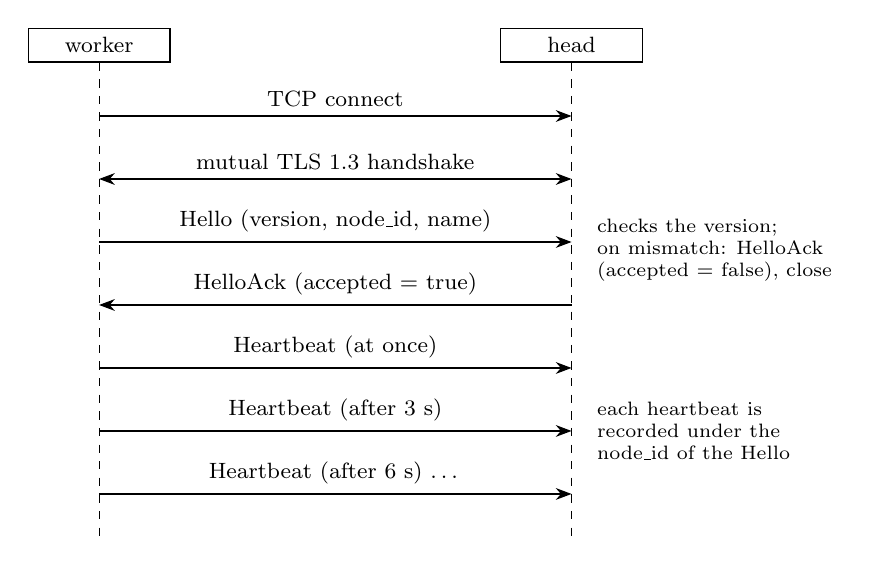
\begin{tikzpicture}[
      font=\footnotesize,
      >={Stealth[length=2mm]},
      note/.style={font=\scriptsize, align=left, anchor=west}]
    \node[draw, minimum width=1.8cm] (w) at (0,0) {worker};
    \node[draw, minimum width=1.8cm] (h) at (6,0) {head};
    \draw[dashed] (w.south) -- (0,-6.3);
    \draw[dashed] (h.south) -- (6,-6.3);
    \draw[->]  (0,-0.9) -- node[above] {TCP connect} (6,-0.9);
    \draw[<->] (0,-1.7) -- node[above] {mutual TLS 1.3 handshake} (6,-1.7);
    \draw[->]  (0,-2.5) -- node[above] {Hello (version, node\_id, name)} (6,-2.5);
    \draw[<-]  (0,-3.3) -- node[above] {HelloAck (accepted = true)} (6,-3.3);
    \draw[->]  (0,-4.1) -- node[above] {Heartbeat (at once)} (6,-4.1);
    \draw[->]  (0,-4.9) -- node[above] {Heartbeat (after 3 s)} (6,-4.9);
    \draw[->]  (0,-5.7) -- node[above] {Heartbeat (after 6 s) \dots} (6,-5.7);
    \node[note] at (6.2,-2.6) {checks the version;\\on mismatch: HelloAck\\(accepted = false), close};
    \node[note] at (6.2,-4.9) {each heartbeat is\\recorded under the\\node\_id of the Hello};
  \end{tikzpicture}
  \caption{A successful connection. After HelloAck the head sends
    nothing more; the channel is one-way.}
  \label{fig:sequence}
\end{figure}

Figure~\ref{fig:sequence} shows a successful connection. Step by step:

\begin{enumerate}
  \item The worker opens TCP to \code{head_addr} and completes the TLS
    handshake. The worker checks that the head's certificate is signed by
    the cluster CA and carries the name \code{clusterd-node}; the head
    checks that the worker's certificate is signed by the cluster CA.
  \item The worker sends \code{Hello} as the first frame.
  \item The head compares \code{protocol_version} with its own. On a
    mismatch it sends, on a best-effort basis, \code{HelloAck} with
    \code{accepted} set to false and a \code{reason}, then closes the
    connection. Otherwise it replies with \code{accepted} set to true. Any
    other first message closes the connection.
  \item The worker starts heartbeating: the first heartbeat immediately,
    then one every \code{heartbeat_interval_secs} (3~s by default). If the
    worker falls behind, missed ticks are delayed rather than sent in a
    burst.
  \item The head records each heartbeat in the node table under the
    \code{node_id} given in \code{Hello}. A heartbeat carrying a different
    \code{node_id} is logged and dropped. Other message types are logged
    and ignored. A frame that cannot be decoded closes the connection.
  \item The connection ends when either side closes it or an error occurs.
    There is no goodbye message: from the head's point of view a closed
    connection and a silently stalled one look the same, and both are
    handled by the same timeout (Section~\ref{sec:updown}). In addition,
    the head closes a connection on which nothing has arrived for
    \code{heartbeat_timeout_secs}: its node is already reported down, and
    without this a peer that vanished without closing (power loss, cable
    pulled) would hold a task and a socket on the head for ever, because
    the head only reads and TCP never reports the loss.
\end{enumerate}

Steps 1 to 3 must complete within 10~seconds (\code{HANDSHAKE_TIMEOUT}),
on both sides, or the connection is dropped. On a local network they take
milliseconds; the bound stops a peer that connects and then says nothing
from holding resources on the head indefinitely.

After \code{HelloAck} the head sends nothing more. The worker reads only
to notice that the connection has closed, and ignores any frame it
receives without decoding it.

\subsection{Message reference}

Phase~1 has three message types. The head's own heartbeat has the same
content as \code{Heartbeat} but is recorded in-process, without going
through the network.

\begin{table}[htbp]
  \centering
  \begin{tabular}{L{0.25\textwidth}L{0.13\textwidth}L{0.5\textwidth}}
    \hline
    Field & Type & Meaning \\
    \hline
    \multicolumn{3}{l}{\emph{Hello} --- worker to head, first frame only} \\
    \hline
    \code{protocol_version} & \code{u16}
      & The sender's \code{PROTOCOL_VERSION}; must equal the head's. \\
    \code{node_id} & UUID v7
      & Stable identity from \code{config.toml}. Every heartbeat on this
        connection is filed under it. \\
    \code{node_name} & string
      & Human-readable name from \code{config.toml}; display only. \\
    \code{cert_fingerprint} & string
      & Reserved for audit logging. The current worker sends an empty
        string and the head ignores the field. \\
    \hline
    \multicolumn{3}{l}{\emph{HelloAck} --- head to worker, reply to Hello} \\
    \hline
    \code{protocol_version} & \code{u16}
      & The head's own version, so a rejected worker can log what was
        expected. \\
    \code{accepted} & \code{bool}
      & False only on a version mismatch. \\
    \code{reason} & optional string
      & Explanation for a human reading the logs; not meant for program
        logic. \\
    \hline
    \multicolumn{3}{l}{\emph{Heartbeat} --- worker to head, on a timer} \\
    \hline
    \code{node_id} & UUID
      & Must equal the \code{node_id} of this connection's
        \code{Hello}. \\
    \code{cpu_free_pct} & \code{f32}
      & 0 to 100; see Section~\ref{sec:telemetry}. \\
    \code{mem_total_bytes} & \code{u64} & Physical memory. \\
    \code{mem_free_bytes} & \code{u64} & Memory available to new work. \\
    \code{disk_free_bytes} & \code{u64}
      & Free space on the filesystem holding the data directory. \\
    \code{running_jobs} & list of UUID & Always empty in Phase~1. \\
    \code{agent_version} & string
      & Package version of the sending binary. \\
    \code{timestamp} & system time
      & The sender's wall clock when sampling. Stored, but neither shown
        nor used for the timeout. \\
    \hline
  \end{tabular}
  \caption{Phase~1 messages.}
  \label{tab:messages}
\end{table}

\subsection{Versioning}

\code{PROTOCOL_VERSION} (currently~1) is incremented on every change to
\code{Message} that breaks the encoding. Because it is checked during the
handshake and must match exactly, a version mismatch fails loudly and
immediately instead of silently misreading bytes on either side.

Adding new variants at the \emph{end} of the enum does not change how the
existing variants are encoded, so the messages planned for Phases~2
and~3 can be added without breaking the Phase~1 ones. This compatibility
is only partial; see Section~\ref{sec:lim-protocol}.

\subsection{Local control protocol}

The command-line program and the agent on the same machine talk over a
Unix-domain socket, \code{clusterd.sock} in the data directory, using
\code{LocalRequest} and \code{LocalResponse} from \path{ipc.rs}. Framing
is the same length-delimited kind, with a 4~MiB limit, carrying bincode.
It is deliberately a different enum and a different codec instance from
the cross-machine protocol: this traffic never leaves the machine, so it
has no versioning or authentication concerns of its own --- access is
governed by filesystem permissions on the socket. Each connection carries
exactly one request and one reply, and only the head runs the server.

\begin{table}[htbp]
  \centering
  \begin{tabular}{L{0.15\textwidth}L{0.4\textwidth}L{0.33\textwidth}}
    \hline
    Request & Reply & Notes \\
    \hline
    \code{Status}
      & \code{Status} with one \code{NodeStatus} per known machine, or
        \code{Error} with a message
      & Backs \code{clusterd status}; answered from the node table. \\
    \hline
  \end{tabular}
  \caption{Local control requests.}
  \label{tab:ipc}
\end{table}

A \code{NodeStatus} contains \code{node_id}, \code{node_name}, \code{up},
\code{last_seen_secs_ago}, the four resource figures, the number of
running jobs and \code{agent_version}; entries are sorted by name.

At start-up the head checks that the socket path fits the operating
system's limit for Unix sockets (107 bytes on Linux, 103 on macOS) and
fails with a clear message otherwise; \code{clusterd init} makes the same
check before writing anything. It then deletes any file already at the
socket path, so that a socket left behind by a crash does not prevent it
from binding. This is safe only because of the data-directory lock: no
other agent can be serving that socket.

% ======================================================================
\section{Failure detection and recovery}
% ======================================================================

\subsection{The up/down rule}
\label{sec:updown}

For each \code{node_id} the head stores the instant at which it
\emph{received} the latest heartbeat --- not the time the sender claims to
have sent it. This instant comes from the head's monotonic clock
(\code{std::time::Instant}), so clock differences between machines and
adjustments of the wall clock have no effect on the decision. When the
table is queried, a machine is \emph{up} if and only if
\[
  \textit{now} - \textit{last received} \le
  \texttt{heartbeat\_timeout\_secs}
\]
(15~s by default; the boundary is inclusive and is tested exactly at
15~s and 16~s). Otherwise \code{clusterd status} reports it as
\code{DOWN}.

\subsection{Detection latency and tolerance}

Let $I$ be the heartbeat interval and $T$ the timeout. A worker that
stops at time $t$ sent its last heartbeat at some time in
$(t - I,\, t\,]$, so it is reported down between $T - I$ and $T$ after it
stopped --- between 12 and 15~seconds with the defaults --- plus network
delay. In the other direction, a machine that is alive but whose
heartbeats are lost or late is reported down only after no heartbeat has
arrived for $T$ seconds; with the defaults it survives about four
consecutive lost heartbeats.

The head's own entry is fed in-process and cannot go down while the head
agent is running.

\subsection{Reconnection}
\label{sec:reconnect}

All retry policy lives in one place, \code{run_worker}. After any
failure the worker waits and tries again. The wait starts at 1~s and
doubles after every failed attempt up to 30~s (1, 2, 4, 8, 16, 30, 30,
\dots~s). If the attempt that just ended had lasted more than 10~s --- that
is, the connection had been healthy --- the wait first goes back to 1~s.
Every kind of failure is retried this way: an unreachable head, a
rejected certificate, a rejected version, missing certificate files, a
handshake that does not finish within 10~s. The worker never exits on
its own.

\subsection{Restart of the head}

When the head agent restarts, its node table starts empty. The head's own
entry reappears immediately; each worker reappears when it reconnects. If
only the head \emph{process} stopped, the operating system closes its
connections, so the workers notice at once and reconnect within their
back-off delay (at most 30~s after the head is ready). If the head
\emph{machine} disappeared, the workers can take much longer to notice
(Section~\ref{sec:lim-availability}).

% ======================================================================
\section{Resource figures}
\label{sec:telemetry}
% ======================================================================

Each heartbeat carries a fresh sample taken by \code{ResourceSampler}
(\path{resources.rs}) on the machine that sends it. Each agent keeps one
sampler for the life of the process, because the CPU figure is a
difference between two consecutive readings.

\begin{table}[htbp]
  \centering
  \begin{tabular}{L{0.24\textwidth}L{0.64\textwidth}}
    \hline
    Field & How it is measured \\
    \hline
    \code{cpu_free_pct}
      & 100 minus the average usage over all cores since the previous
        sample, as computed by \code{sysinfo}, clamped to 0--100. Two
        readings are always at least 200~ms apart (the minimum for a
        meaningful figure); the first sample after start-up waits out
        that interval. \\
    \code{mem_total_bytes}
      & Total physical memory. \\
    \code{mem_free_bytes}
      & \emph{Available} memory (\code{MemAvailable} on Linux): memory
        that can be given to new work without swapping, including
        reclaimable cache. This is the right figure for placement
        decisions, rather than the kernel's strict ``free'' memory. \\
    \code{disk_free_bytes}
      & Space available on the filesystem whose mount point is the longest
        prefix of the data-directory path. The path is first resolved to
        an absolute path without symbolic links, the form in which mount
        points are given. In Phase~4 this will be the dedicated storage
        volume instead. \\
    \code{running_jobs}
      & Always empty until Phase~2. \\
    \hline
  \end{tabular}
  \caption{How the resource figures are obtained.}
  \label{tab:telemetry}
\end{table}

% ======================================================================
\section{Operations}
% ======================================================================

\subsection{Command-line interface}

All commands accept the global option \code{--data-dir}; its default is
\path{./clusterd-data}, relative to the current directory.

\begin{verbatim}
clusterd init --node-name N --role head --listen IP:PORT
clusterd init --node-name N --role worker --head IP:PORT
clusterd cert issue --name N --out DIR
clusterd agent run
clusterd status
\end{verbatim}

\begin{description}
  \item[init (head)]
    Creates the data directory, writes \code{config.toml} with a new
    \code{node_id}, creates the cluster CA and the head's own certificate,
    and prints the next steps. Refuses a directory that is already
    initialised (it would replace the CA and cut off every worker), and
    one whose control-socket path would be too long.
  \item[init (worker)]
    Writes \code{config.toml} only. The worker's certificate files are
    copied in afterwards. Refuses a directory that is already
    initialised.
  \item[cert issue]
    Run against the head's data directory. Writes \code{ca.crt},
    \code{node.crt} and \code{node.key} for a new machine into
    \code{DIR}, which must not be the head's own data directory.
  \item[agent run]
    Runs the agent in the foreground.
  \item[status]
    Run on the head. Prints one line per known machine with the columns
    NAME, UP, CPU FREE, MEM TOTAL, MEM FREE, DISK FREE, JOBS, VERSION and
    LAST SEEN.
\end{description}

Addresses are parsed as a numeric IP address and port; host names are not
accepted.

\subsection{Data directory}

\begin{table}[htbp]
  \centering
  \begin{tabular}{L{0.2\textwidth}L{0.17\textwidth}L{0.51\textwidth}}
    \hline
    File & Present on & Content \\
    \hline
    \code{config.toml} & every machine
      & Role, \code{node_id}, name, address, heartbeat timing \\
    \code{ca.crt} & every machine & Cluster CA certificate \\
    \code{ca.key} & head only & Cluster CA private key, mode \code{0600} \\
    \code{node.crt} & every machine
      & This machine's certificate, signed by the cluster CA \\
    \code{node.key} & every machine
      & This machine's private key, mode \code{0600} \\
    \code{clusterd.sock} & head only
      & Local control socket, created while the agent runs \\
    \code{clusterd.lock} & every machine
      & Locked by the running agent, so that only one agent at a time uses
        the directory \\
    \hline
  \end{tabular}
  \caption{Files in the data directory.}
  \label{tab:datadir}
\end{table}

A worker's \code{config.toml} looks like this:

\begin{verbatim}
node_id = "01a1b7cc-1e8a-7d92-9525-907b9c27ba73"
node_name = "worker-1"
role = "worker"
head_addr = "192.168.1.10:7700"
heartbeat_interval_secs = 3
heartbeat_timeout_secs = 15
\end{verbatim}

A head has \code{listen_addr} instead of \code{head_addr}. The file is
validated whenever it is loaded: the interval must be at least 1~s and
the timeout greater than the interval. The interval is used by the
machine that sends heartbeats; the timeout is used only by the head, so
keep the head's timeout well above every worker's interval. Once systemd
packaging exists (Phase~3), the data directory should move to
\path{/var/lib/clusterd}.

\subsection{Logs}

The log level is set with the \code{RUST_LOG} environment variable
(default \code{info}). On Linux, if the systemd journal is reachable ---
which is the case on any systemd distribution, including in an interactive
SSH session --- logs go \emph{only} to the journal, under the name of the
executable:

\begin{verbatim}
journalctl -t clusterd -f
\end{verbatim}

Elsewhere (macOS, containers without a journal) logs go to standard
error. Command output, such as the status table, always goes to standard
output.

\subsection{Local smoke test}

\path{bin/dev-smoke-test.sh} is a manual, human-readable demonstration on
one machine. It builds the debug binary, creates fresh data directories
under \path{data/smoke-test} in the repository, starts a head on
\code{127.0.0.1:17700} and two workers as separate processes, waits 5~s
and prints \code{status} (all three up), stops one worker, waits 17~s and
prints \code{status} again (that worker \code{DOWN}, the others up). It
proves the logic, not real networking between hosts.

\subsection{Deploying on real machines}

The smoke test and the automated integration test prove the logic. Only
separate hosts prove that real TCP, real TLS between different machines
and real \code{sysinfo} readings on Ubuntu behave as expected. The
procedure below uses Ubuntu Server virtual machines.

\paragraph{Building the binary.}
The development Mac has no Linux cross-compilation toolchain: ring, the
crypto backend, needs a C cross-compiler for Linux, and getting one that
matches the target machines' C library is a project of its own. The
reliable path is to build natively on one of the Ubuntu machines and copy
the resulting executable to the others. Any machine can serve as build
machine, including the head.

\paragraph{1. Copy the source to the build machine.} From the Mac:
\begin{verbatim}
cd /Users/paul/myFiles/PROJECTS/PRIO01_Minimal_Distibuted_System
rsync -avz --exclude target --exclude data --exclude log \
  ./ <user>@<build-vm-ip>:~/clusterd/
\end{verbatim}
Pushing the repository to a Git remote and cloning it on the machine
works equally well.

\paragraph{2. Install Rust and a C toolchain on the build machine.}
\begin{verbatim}
ssh <user>@<build-vm-ip>
sudo apt update && sudo apt install -y build-essential pkg-config
curl --proto '=https' --tlsv1.2 -sSf https://sh.rustup.rs \
  | sh -s -- -y
source "$HOME/.cargo/env"
\end{verbatim}

\paragraph{3. Build the release binary.}
\begin{verbatim}
cd ~/clusterd
cargo build --release -p clusterd
ls -la target/release/clusterd
\end{verbatim}
\path{target/release/clusterd} is the only file the other machines need.

\paragraph{4. Copy the binary to every other machine.}
\begin{verbatim}
for host in <worker-vm-1-ip> <worker-vm-2-ip>; do
  scp target/release/clusterd <user>@$host:~/clusterd
done
\end{verbatim}
No Rust toolchain is needed on the workers.

\paragraph{5. Set up the head.} On the machine chosen as head:
\begin{verbatim}
./clusterd --data-dir ~/clusterd-data init \
  --node-name head-1 --role head --listen 0.0.0.0:7700
\end{verbatim}
This creates the cluster CA and the head's certificate. Note the head's
IP address; workers need it. If \code{ufw} is active, open the port with
\code{sudo ufw allow 7700/tcp}.

\paragraph{6. Issue a certificate for each worker.} Still on the head:
\begin{verbatim}
./clusterd --data-dir ~/clusterd-data cert issue \
  --name worker-1 --out ~/worker-1-certs
./clusterd --data-dir ~/clusterd-data cert issue \
  --name worker-2 --out ~/worker-2-certs
scp ~/worker-1-certs/* <user>@<worker-vm-1-ip>:~/worker-1-certs/
scp ~/worker-2-certs/* <user>@<worker-vm-2-ip>:~/worker-2-certs/
\end{verbatim}

\paragraph{7. Set up each worker.} On each worker, with its own name and
directory:
\begin{verbatim}
./clusterd --data-dir ~/clusterd-data init \
  --node-name worker-1 --role worker --head <head-vm-ip>:7700
cp ~/worker-1-certs/* ~/clusterd-data/
\end{verbatim}
Run \code{init} on each machine itself, after any cloning of virtual
machines; a copied data directory duplicates the \code{node_id}
(Section~\ref{sec:lim-availability}).

\paragraph{8. Start the agents.} Until Phase~3 installs systemd services,
run the agents under \code{tmux} or \code{screen} so they survive the
end of the SSH session. On the head and on every worker:
\begin{verbatim}
RUST_LOG=info ./clusterd --data-dir ~/clusterd-data agent run
\end{verbatim}
The terminal stays silent: logs go to the journal. Follow them from a
second session with \code{journalctl -t clusterd -f}.

\paragraph{9. Check the pool from the head.} In another session on the
head:
\begin{verbatim}
./clusterd --data-dir ~/clusterd-data status
\end{verbatim}
Every machine should be listed as up, with live figures.

\paragraph{10. Check down detection.} Stop the agent on one worker
(Ctrl-C or \code{kill}), wait about 15~s, and run \code{status} again on
the head. That worker should be \code{DOWN}; the others stay up.

\subsection{Troubleshooting}

\begin{itemize}
  \item \textbf{No log output at all.}
    On Linux the logs are in the journal: \code{journalctl -t clusterd}.
  \item \textbf{status fails with ``is clusterd agent run running on this
    host?''.}
    Either the agent is not running on this machine; or \code{--data-dir}
    differs from the one the agent was started with; or this is a worker
    (only the head serves \code{status}).
  \item \textbf{``another clusterd agent is already running''.}
    An agent is already using this data directory; stop it first. (Two
    agents on one data directory would share one identity.)
  \item \textbf{A worker never appears in the status.}
    Check that the head's firewall accepts TCP on the \code{--listen}
    port, and that the worker can reach the head: run
    \code{nc -zv <head-vm-ip> 7700} on the worker. Then read the worker's
    log.
  \item \textbf{``invalid peer certificate'' or ``received fatal alert''
    in the logs.}
    The two sides do not trust the same CA. Check that \code{ca.crt},
    \code{node.crt} and \code{node.key} in the worker's data directory are
    the files \code{cert issue} produced on \emph{this} cluster's head.
  \item \textbf{``head rejected connection: protocol version mismatch''.}
    Head and worker run binaries with different protocol versions; copy
    the same binary everywhere.
  \item \textbf{``already initialised''.}
    \code{init} refuses to replace an existing identity. To really start
    over on that machine, delete its data directory first. On the head
    this creates a new CA, and every worker then needs a new
    certificate.
  \item \textbf{A removed or re-initialised machine is still listed as
    DOWN.}
    The node table never forgets an entry
    (Section~\ref{sec:lim-availability}). Restart the head agent to
    clear it.
\end{itemize}

% ======================================================================
\section{Verification}
% ======================================================================

As of 7~November~2026, the following commands all succeed cleanly:

\begin{itemize}
  \item \code{cargo build --workspace};
  \item \code{cargo test --workspace}: 50 tests, all passing;
  \item \code{cargo clippy --workspace --all-targets}: no warnings;
  \item \code{cargo fmt --all -- --check}: no differences.
\end{itemize}

The repository has no continuous-integration configuration; these
commands are run by hand.

\begin{table}[htbp]
  \centering
  \begin{tabular}{L{0.24\textwidth}L{0.07\textwidth}L{0.57\textwidth}}
    \hline
    Suite & Tests & What it covers \\
    \hline
    \code{clusterd-proto} unit & 9
      & Round trip of every variant; rejection of every truncation of a
        heartbeat, of garbage, of empty input and of oversized input;
        framed round trip over an in-memory stream; rejection of an
        oversized length prefix by the codec; readable error messages;
        property-based test that decoding arbitrary bytes never
        panics. \\
    \code{clusterd-core} unit & 34
      & Configuration round trip and validation, including heartbeat
        timing; full cause chains in error messages; CA and certificate
        generation, and that rustls can load the result; private keys
        written with mode \code{0600}, also over an existing wider file;
        building matching server and client TLS configurations; readable
        errors for missing or empty PEM files; node-table up/down at and
        past the timeout boundary, reset by a later heartbeat, sorting;
        resource figures within range, with a relative data directory,
        and a real CPU reading in the first sample; control-socket path
        limit and replacement of a stale socket file. \\
    \code{clusterd} unit & 4
      & \code{init} refuses an initialised directory and a too-long
        socket path; \code{cert issue} refuses the head's data directory
        and writes its three files elsewhere. \\
    Integration (\path{tests/integration.rs}) & 3
      & Over real localhost TCP and TLS, with a 1~s interval and 2~s
        timeout: a worker joins and both are up, then is stopped and flips
        to down while the head stays up; a second agent on the same data
        directory is refused while the first keeps serving status; the
        head closes a connection that goes silent after the
        handshake. \\
    \hline
  \end{tabular}
  \caption{Automated tests.}
  \label{tab:tests}
\end{table}

In addition, \path{bin/dev-smoke-test.sh} demonstrates the same scenario
with three processes on one machine, and the procedure of the previous
section validates it on separate machines. The gaps in this coverage are
listed in Section~\ref{sec:lim-testing}.

% ======================================================================
\section{Limitations}
\label{sec:limitations}
% ======================================================================

This section lists what the current design does not do or does poorly.
For each item it states the consequence and what would address it.
Plain bugs found while writing this document have been fixed; they are
recorded in Section~\ref{sec:defects}.

\subsection{Scope of Phase 1}

\paragraph{Monitoring only.}
Phase~1 observes the pool; it does not use it. No job can be submitted,
placed or run; \code{running_jobs} is always empty and the JOBS column is
always~0.

\paragraph{Manual onboarding.}
Adding a worker takes several manual steps on two machines: issue a
certificate on the head, copy three files, run \code{init} on the worker,
start the agent. Phase~3's \code{clusterd join} is meant to reduce this
to one command run on the head.

\paragraph{No storage pooling.}
Nothing in Phase~1 touches storage; disk space is only reported.

\paragraph{No service management and no orderly shutdown.}
The agent is a foreground process: it does not restart after a crash and
does not start at boot. It handles no signals; Ctrl-C or \code{SIGTERM}
end it immediately. No work is lost today, but the control socket file is
left behind (it is removed at the next start). Phase~3 installs systemd
units; orderly shutdown will matter from Phase~2, when a stopping worker
has jobs running.

\paragraph{One run per machine, by design.}
As stated in the introduction, an individual run is limited to the
resources of one machine. This is a permanent property of the design,
not a temporary gap.

\paragraph{Small scale, one local network.}
The design assumes a handful to a few tens of machines on one trusted
local network: all heartbeats converge on the head, through one mutex,
over one connection per worker. It has not been designed or measured for
wide-area networks or for hundreds of machines; the automated and
scripted tests use at most three.

\subsection{Availability and fault tolerance}
\label{sec:lim-availability}

\paragraph{The head is a single point of failure.}
Without the head there is no status, and in later phases there will be no
scheduling and no storage master either; workers just keep trying to
reconnect. Nothing on the head is replicated. This is accepted for now.
For storage, SeaweedFS supports multiple masters with Raft natively, so
that part is a bounded upgrade later; making the scheduler redundant is a
separate, harder problem.

\paragraph{The head's address must be fixed and numeric.}
Each worker stores the head's IP address and port; host names are not
accepted. If the head's address changes, every worker's
\code{config.toml} must be edited. Give the head a static address or a
DHCP reservation.

\paragraph{Workers are slow to notice a head machine that disappears.}
After \code{HelloAck} the head never sends anything, and no TCP
keep-alive is configured. If the head \emph{process} stops, its operating
system closes the connections and workers notice at once. But if the
head \emph{machine} loses power or network, a worker keeps writing
heartbeats into its socket buffer and only learns that the connection is
dead when TCP gives up retransmitting --- about 15~minutes with Linux
defaults. If the head comes back earlier, its kernel answers the next
retransmission with a reset; since retransmissions back off exponentially
(up to two minutes apart on Linux), a worker can still stay absent from
\code{status} for minutes after the head is back. An application-level
reply from the head, or TCP keep-alive, would bound this to a few
heartbeat intervals.

\paragraph{The node table never forgets.}
There is no command to remove a machine. A decommissioned machine, or one
whose data directory was re-initialised (which creates a new
\code{node_id}), stays in \code{status} as \code{DOWN} until the head
restarts.

\paragraph{Duplicate identities are not detected.}
If a virtual machine is cloned after \code{init}, both copies share the
same \code{node_id} (and the same certificate). Their heartbeats
overwrite each other in one row, which then alternates between the two
machines' figures, and the pool appears smaller than it is. Two machines
may also carry the same \code{node_name}; nothing checks that names are
unique.

\paragraph{Failure detection is timeout-only and binary.}
``Down'' means only ``no heartbeat received for 15~s''. A crashed
machine, a network partition and a machine so overloaded that its agent
misses heartbeats all look the same. In Phase~2 a false ``down'' could
cause a job to be started twice; the scheduler will have to treat ``down''
as ``unknown'', not as ``dead''.

\subsection{Security}
\label{sec:lim-security}

\paragraph{Machine identity is self-declared.}
The head admits any connection with a valid cluster certificate and then
takes \code{node_id} and \code{node_name} from the \code{Hello} message
as given. The check on later heartbeats only stops a connection from
switching identity midway. Consequently, anyone holding any one valid
cluster certificate can register as any machine: overwrite another
machine's row with false figures, imitate the head's own
\code{node_id}, or open many connections with invented identifiers to
fill the table. The \code{cert_fingerprint} field, intended for this kind
of check, is sent empty and ignored. The fix is to bind identity to the
certificate --- for example, put the \code{node_id} in the certificate at
issue time and reject a \code{Hello} that does not match it.

\paragraph{Head and worker certificates are interchangeable.}
Every machine certificate carries the same name, \code{clusterd-node},
and no extended-key-usage restriction, so any worker's certificate is
also a valid \emph{head} certificate. Someone who has a worker's private
key and can divert traffic on the local network (for example by ARP
spoofing) can impersonate the head to the other workers. Today the impact
is limited to monitoring data. From Phase~2, when the head sends jobs,
impersonating the head would mean running arbitrary commands on every
worker. Before Phase~2 the head needs a distinct identity (a different
name or usage in its certificate) that workers require.

\paragraph{No revocation and no expiry.}
Certificates are valid from 1975 to 4096, and there is no revocation list.
A certificate, once issued, admits its holder for good. The only way to
exclude a lost or compromised machine is to create a new CA and reissue
every certificate. Short-lived certificates renewed automatically, or a
revocation list checked by the head, would address this; Phase~3's
automated join is the natural place.

\paragraph{The CA key is online and unprotected beyond file permissions.}
\code{ca.key} sits unencrypted on the head, which is also a working
machine of the pool. Whoever obtains it can issue certificates at will;
compromising the head therefore compromises the whole cluster. The CA is
also unconstrained (no limit on path length, no name constraints). Moving
the CA key offline, or encrypting it with a passphrase needed only when
issuing, would reduce this.

\paragraph{The listener has no connection limit.}
Connections that don't finish the handshake are dropped after 10~s,
silent ones after the heartbeat timeout, and a failed \code{accept} no
longer stops the head. But there is still no limit on the number of
simultaneous connections: anyone who can reach the port can keep opening
connections, each holding a task and a file descriptor for up to 10~s,
and while the process is out of file descriptors legitimate workers
cannot connect either. A peer with a valid certificate can also send
frames of up to 16~MiB, far beyond the roughly hundred bytes a heartbeat
needs. A connection limit set below the process's file-descriptor limit,
and a much smaller frame limit, would close this.

\paragraph{Reported figures are trusted as given.}
The head does not check the figures it receives: a CPU percentage outside
0--100 or not a number, more free memory than total memory, and so on,
are stored and displayed as they are. This matters from Phase~2, when the
scheduler will base decisions on them.

\paragraph{Local socket permissions are implicit.}
\code{clusterd.sock} and the data directory get whatever permissions the
process's umask produces; clusterd sets none explicitly. Anyone who can
connect to the socket can read the status. That is harmless today, but
Phase~2 commands such as \code{run} over the same socket would need
explicit permissions or a peer-credential check.

\paragraph{Not audited.}
None of this has had an independent security review.

\subsection{Protocol evolution}
\label{sec:lim-protocol}

\paragraph{Upgrades must be done all at once.}
The protocol version must match exactly, and there is no negotiation of
capabilities. Whenever \code{PROTOCOL_VERSION} changes, the head and all
workers must be upgraded together; a rolling upgrade is impossible.

\paragraph{``Additive'' changes are compatible in one direction only.}
bincode is not self-describing: adding, removing or reordering a field of
an existing message always breaks the encoding. Appending a new message
type is safe only if the head is upgraded first, because an older head
that receives a type it does not know fails to decode the frame and
closes the connection. (An older worker ignores everything it receives
after the handshake, so it does not mind.) Note also that bincode's
default configuration accepts trailing bytes after a valid message, so
decoding is not a strict validation of the frame.

\paragraph{The channel is one-way today.}
The head sends nothing after \code{HelloAck}, and the worker does not
decode what it receives. Phase~2 needs the head to send jobs, so the
worker side will have to start decoding messages, and both sides will
have to handle unknown types gracefully.

\subsection{Accuracy of the resource figures}

\paragraph{One CPU percentage is not comparable between machines.}
The figure is an average over all cores, and the core count is not
reported. ``50~\% free'' means one core on a two-core machine and eight
cores on a sixteen-core one. The scheduler will need the number of cores,
and probably the load average, in the heartbeat --- a protocol change.

\paragraph{Disk figure.}
The disk figure is the free space of the filesystem holding the data
directory, which may have nothing to do with the space the pool will use.

\paragraph{Timestamps.}
The sender's timestamp is stored but neither shown nor used, and
``last seen'' is rounded down to whole seconds.

\paragraph{Linux only.}
Only Linux is a target platform. On macOS, used for the local smoke test,
\code{MEM FREE} was observed as 0; the smoke test there validates the
logic, not the figures.

\subsection{Operability}

\paragraph{Logs are not where people look.}
On Linux, logs go only to the journal (when it is reachable), even when
the agent is run by hand in a terminal, which then stays silent. Step~8
of the deployment procedure is the first place where this surprises.
Writing to standard error as well when attached to a terminal would avoid
the surprise.

\paragraph{Misconfiguration does not fail fast.}
A worker with missing or wrong certificate files, or a wrong head
address, does not stop: it retries for ever with back-off and logs a
warning each time. The warning gives the cause, but nothing stops the
agent or alerts anyone; someone has to read the journal.

\paragraph{status works only on the head.}
On a worker, \code{clusterd status} fails with a message suggesting the
agent is not running, although it is.

\paragraph{Heartbeat settings are checked per machine only.}
Each machine checks its own \code{config.toml} (interval at least 1~s,
timeout greater than the interval). But the two values that interact live
on different machines --- the interval on each worker, the timeout on the
head --- and nothing checks them against each other. A worker whose
interval is close to or above the head's timeout flaps between up and
down, and the head closes its connection between heartbeats.

\paragraph{The head reads its certificates once.}
A worker reloads its certificate files on every connection attempt, so
new files take effect at the next reconnection. The head loads them only
at start-up; changing them requires a restart.

\paragraph{The binary is not static.}
The executable is self-contained apart from the system C library (glibc).
It must be built against a glibc no newer than that of the oldest target
machine, which is why it is built natively on one of the target machines.
A static (musl) build or cross-compilation from the Mac would remove this
constraint later.

\paragraph{No health or metrics interface.}
\code{clusterd status} is the only view into the system. There is no
machine-readable output, no health endpoint and no metrics export.

\subsection{Testing}
\label{sec:lim-testing}

\paragraph{Fixed ports.}
Two integration tests use fixed ports (18700 and 18702), and the smoke
test uses 17700; they fail if the port is in use.

\paragraph{Untested paths.}
No automated test covers reconnection and back-off, rejection of a
version mismatch end to end, rejection of a certificate from another CA,
identity spoofing, the handshake timeout, recovery from a failed
\code{accept}, or behaviour across separate machines. All the defects of
Section~\ref{sec:defects} lay in paths that had no test at the time.

\paragraph{Timing-dependent scripts.}
The smoke test relies on fixed sleeps and can give false results on a
heavily loaded machine. The integration test polls with a deadline
instead, which is more robust.

\paragraph{No continuous integration.}
Tests are run by hand; nothing prevents a regression from being
committed.

% ======================================================================
\section{Defects found and fixed}
\label{sec:defects}
% ======================================================================

The defects below were found while writing this document, on
7~November~2026. D1 to D4 and D8 were reproduced by running the binary
(macOS development machine); D5 to D7 followed from reading the code and
standard Unix behaviour. All are fixed, each with a regression test unless
stated otherwise, and the reproductions were run again against the fixed
binary. Four related problems that had first been listed as limitations
were fixed at the same time; they close the section.

\paragraph{D1. Disk space was reported as zero with a relative data directory.}
\begin{description}
  \item[Symptom] DISK FREE showed \code{0.0B}, including with the default
    \code{--data-dir ./clusterd-data}.
  \item[Cause] The free-space lookup compares the data-directory path with
    each mount point using \code{Path::starts_with}, which compares whole
    path components. A relative path never starts with an absolute mount
    point, so no filesystem matched and the lookup fell back to~0. A path
    through a symbolic link had the same problem.
  \item[Fix] \code{ResourceSampler::new} resolves the path once to an
    absolute path without symbolic links (\code{canonicalize}).
\end{description}

\paragraph{D2. A second agent on the same data directory broke status for the first.}
\begin{description}
  \item[Symptom] After an accidental second \code{clusterd agent run} on
    the head's data directory, which exited with ``Address already in
    use'', \code{status} failed with ``connection refused'' although the
    first agent was still running.
  \item[Cause] The control-socket server removed any existing file at the
    socket path before binding (meant for files left by a crash), and it
    started before the TCP listener was bound. The second agent deleted the
    live socket, created its own, then failed on the TCP port and exited.
  \item[Fix] Every agent takes an exclusive lock on \code{clusterd.lock}
    in its data directory at start-up; a second agent stops at once with
    ``another clusterd agent is already running''. The head also binds
    both listeners before starting anything else.
\end{description}

\paragraph{D3. Agent logs dropped the cause of errors.}
\begin{description}
  \item[Symptom] A worker presenting a certificate from another CA produced
    only \code{error=io error}, on both sides.
  \item[Cause] Errors were logged with the display text of the top-level
    error only, and the text of the \code{Io} variant is just ``io
    error''.
  \item[Fix] The agent logs \code{Error::chain}, which appends every
    underlying cause. The same situation now reads
    \code{io error: invalid peer certificate: BadSignature} on the worker
    and \code{io error: received fatal alert: DecryptError} on the head.
\end{description}

\paragraph{D4. A long data-directory path silently disabled status.}
\begin{description}
  \item[Symptom] The head ran and workers connected, but \code{status}
    failed with ``path must be shorter than SUN\_LEN''.
  \item[Cause] A Unix socket path is limited to 107 bytes on Linux and 103
    on macOS. The bind failure was logged and the head carried on without
    a control socket.
  \item[Fix] \code{clusterd init} checks the path length before writing
    anything, and the agent checks it again at start-up; the message gives
    the length, the limit and the remedy. Any other failure to bind the
    control socket now stops the agent.
\end{description}

\paragraph{D5. A failed accept stopped the head.}
\begin{description}
  \item[Cause] An error from \code{accept} was propagated out of the
    accept loop, which ended the agent. Accept fails transiently, notably
    when the process runs out of file descriptors --- which anyone able to
    reach the port could provoke.
  \item[Fix] The error is logged and accepting resumes after 100~ms; the
    control-socket server does the same. No automated test: provoking the
    failure would mean exhausting the test process's file descriptors.
\end{description}

\paragraph{D6. A heartbeat interval of zero panicked.}
\begin{description}
  \item[Cause] The interval went straight to \code{tokio::time::interval},
    which panics on a zero period.
  \item[Fix] Configuration validation, applied on every load, requires an
    interval of at least 1~s and a timeout greater than the interval.
\end{description}

\paragraph{D7. Key-file permissions were not enforced when a file already existed.}
\begin{description}
  \item[Cause] The key was written by opening the target with mode
    \code{0600}, but that mode only applies when a file is created; an
    existing file kept its wider permissions with the new key inside.
  \item[Fix] \code{identity::write_secret} writes to a new \code{0600}
    file and renames it over the target.
\end{description}

\paragraph{D8. cert issue into the head's data directory destroyed the CA certificate.}
\begin{description}
  \item[Symptom] \code{clusterd cert issue --out} pointing at the head's
    own data directory left \code{ca.crt} empty and replaced the head's
    certificate and key with the new node's.
  \item[Cause] Copying \code{ca.crt} onto itself truncates it before it is
    read.
  \item[Fix] \code{cert issue} refuses an output directory that resolves
    to the head's data directory.
\end{description}

\paragraph{Fixed at the same time.}
\begin{itemize}
  \item \emph{Wrong first CPU reading.} A new sampler was created for
    every connection, and its first reading, sent immediately, always
    reported the CPU as 100~\% free. There is now one sampler per process,
    and two readings are never less than 200~ms apart.
  \item \emph{Silent connections leaked on the head.} The head now closes
    a connection on which nothing has arrived for the heartbeat timeout.
  \item \emph{No handshake timeout.} TCP connect, TLS and the
    \code{Hello} exchange must now complete within 10~s, on both sides.
    No automated test: it would add 10~s to the test suite.
  \item \emph{init overwrote an existing identity.} \code{clusterd init}
    now refuses a data directory that already holds \code{config.toml} or
    \code{ca.key}.
\end{itemize}

% ======================================================================
\section{Roadmap}
% ======================================================================

\subsection{Phase 2: job submission and scheduling}

Planned: \code{clusterd run} to submit a job from the head, placement on
a machine with free capacity, streaming of the job's output back to the
head, and job history and queue persisted in SQLite (\code{state.db}).
New messages: \code{JobAssign}, \code{JobCancel}, \code{JobStarted},
\code{JobLogChunk}, \code{JobResult}, appended to the enum.

Phase~2 turns ``impersonate a machine'' into ``run code on the cluster'',
so several limitations above become prerequisites rather than
improvements. In order of importance:

\begin{enumerate}
  \item Bind machine identity to the certificate
    (Section~\ref{sec:lim-security}).
  \item Give the head a certificate identity that workers' certificates
    cannot provide, and have workers require it.
  \item Bound the listener further: a connection limit and a smaller
    frame limit (the timeouts and a non-fatal accept loop are in
    place).
  \item Validate reported figures; add the core count (and probably the
    load average) to \code{Heartbeat}, with a protocol version change.
  \item Make the worker decode messages after the handshake and handle
    unknown types gracefully; add an application-level reply so that
    workers detect a vanished head quickly.
  \item Add automated tests for the untested paths of
    Section~\ref{sec:lim-testing}, and set up continuous integration.
\end{enumerate}

\subsection{Phase 3: automated join}

Planned: \code{clusterd join}, run on the head, which uses \code{ssh}
and \code{scp} to copy the binary and a fresh certificate to a new
machine, initialise it, and install and start a systemd unit. Node
registration, implicit today through \code{Hello}, will be formalised
with \code{NodeJoin} and \code{NodeJoinAck} messages. This phase needs
root on the target machines; the aim is narrow capabilities or a scoped
helper rather than a root agent. It is also the natural place for
removing a machine and for revoking or renewing certificates.

\subsection{Phase 4: storage orchestration}

Planned: generate SeaweedFS configuration, run its master and volume
servers under systemd, and mount the pooled storage with FUSE on every
machine. The disk figure will then report the storage volume rather than
the data directory. How SeaweedFS's replication and erasure-coding options
map onto the requirement ``lose one disk or one machine without losing
data'' is to be settled in this phase. SeaweedFS supports several masters
coordinated by Raft, which offers a path out of the head being a single
point of failure for storage.

\end{document}
